\section{Scaling Performance of $512^3$ problem}
Let us proceed now showing the performances achieved by our code in a large sized problem.
The present simulation shown a better scaling effectiveness and efficiency for both methods with respect to $256^{3}$ problem. 
\par
The best results are reached using 8 cores per processor, indicating that the efficiency lack cost overcome the message passing price.
In theory we would rather to use a pure MPI approach instead of a heavily threaded ones, because the speedup achieved by the first method are significantly faster than the latter ones in our implementation. However, for costing reasons, a tradeoff between the two solutions is preferred. \\
\par
The speedup peak is remarkable, with a factor above $430$ on $2048$ cores using pencil decomposition, while stops around $50$ using $128$ cores and slab decomposition. \\
\par

\begin{figure}
\begin{center}
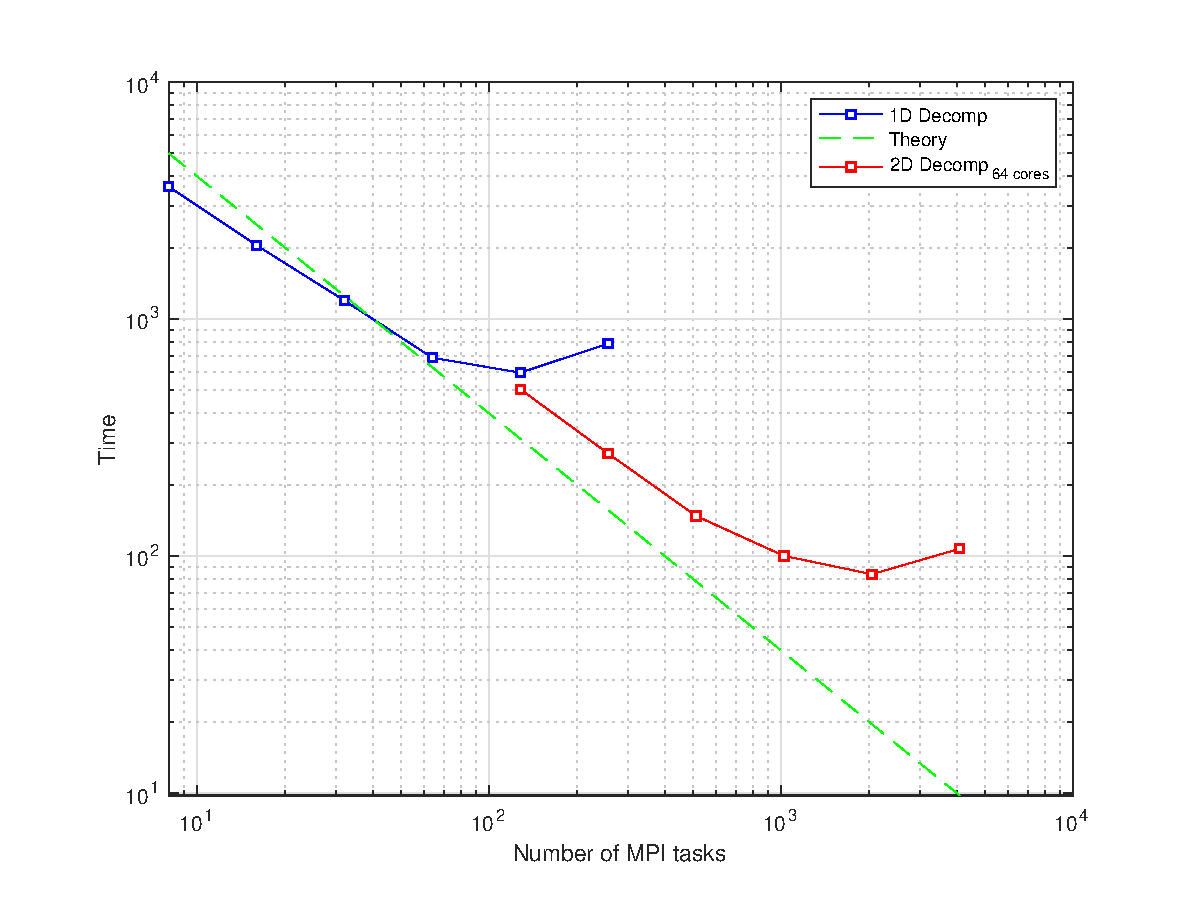
\includegraphics[scale=0.6]{grafici/5121}
\caption{Scaling performance of $512^3$ simulation}
\label{5121}
\end{center}
\end{figure}

\begin{figure}
\begin{center}
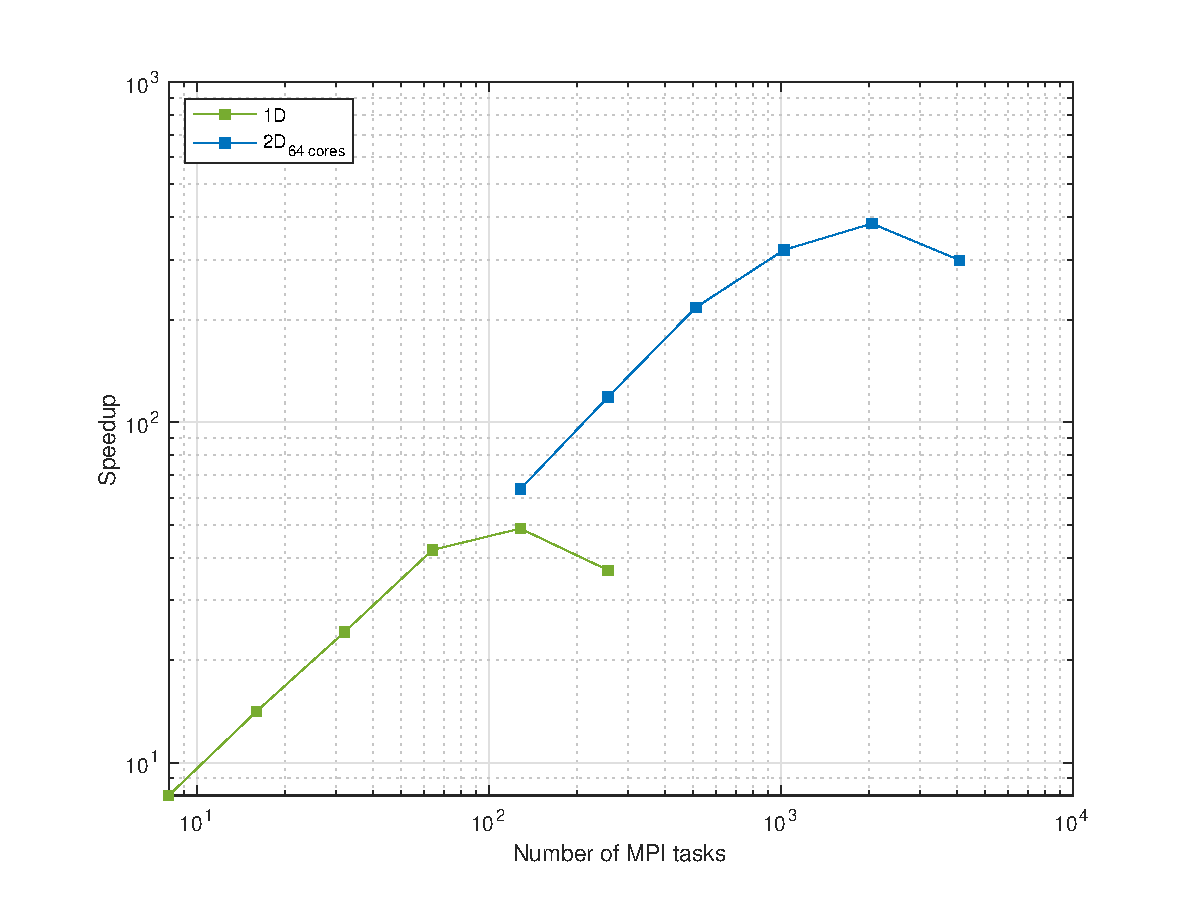
\includegraphics[scale=0.6]{grafici/5122}
\caption{Speedup factor of $512^3$ simulation}
\label{5122}
\end{center}
\end{figure}

\begin{figure}
\begin{center}
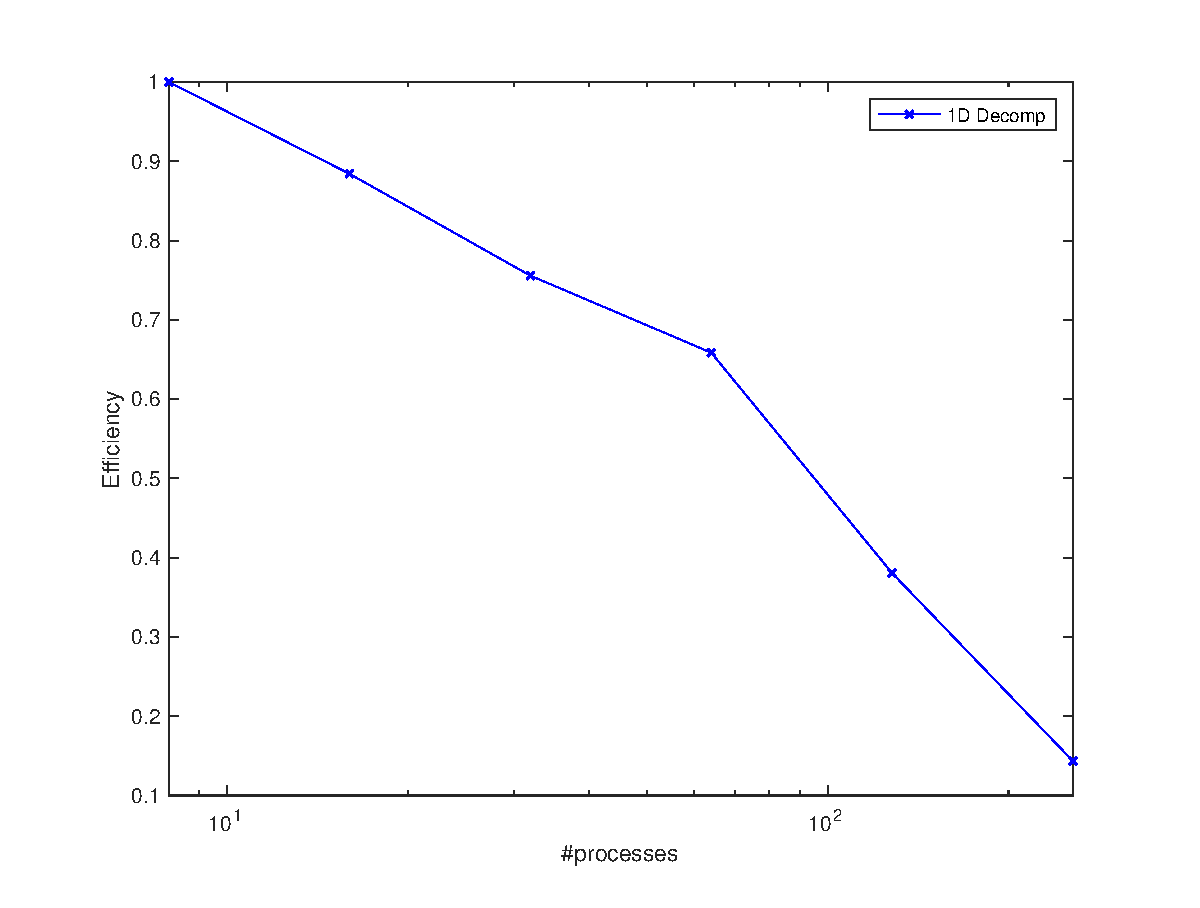
\includegraphics[scale=0.6]{grafici/5123}
\caption{Efficiency factor of $512^3$ simulation using 1D decomposition}
\label{5123}
\end{center}
\end{figure}

As we can see from figure~\ref{5122}, where is compared the slab decomposition against the pencil ones running on 64 cores per processor, the speedup factor of the latter algorithm increase approximately linearly until $512$ cores. The raise in performance continue at lower factor until $2048$ cores are reached, where performances start decreasing. For what concern the first algorithm we face a sub-optimal linear increase in performances until 64 cores are reached. 
The inverse behaviors are shown in figure~\ref{5121}, where the simulation time is plotted against the number of processes.
\par
We refer to figure~\ref{5123} of page~\pageref{5123} to have an idea of the efficiency of the 1D decomposed algorithm. The figure shows that the efficiency remains near the $80\%$ until $32$ cores are used. However, once passed such limit, the behavior is still linear and less sloping with  respect to the ones shown in figure~\ref{1283} of page~\pageref{1283}.  \\
\par
It is interesting to denote how advantageous the 2D decomposed algorithm is; it is clear by looking at the figure~\ref{5121}. The time saving could be in the order of magnitude of $\mathcal{O}(10)$ if compared with the 1D decomposed ones.\\
\par
It is evident that the pencil decomposition outclass the slab ones. However we could improve our results by selecting the proper number of threads per processor. 
\par
Since the $256^{3}$ simulation highlighted that the slab decomposition is less sensitive to the cores per nodes optimization, we decided to skip it and directly pass to analyze the pencil ones. \par
Since the problem dimensions are relevant, the single core analysis can not be carried out because we face an out of memory error.
To decide what is the best solution in terms of 2D decomposition we must evaluate the performances in an homogeneous way. 
By looking at the values in table~\ref{512data:multi} of page~\pageref{512data:multi} and the depicted counter part, in figures~\ref{512:perf} and \ref{512:times} of page~\pageref{512:perf}, it is evident that the single core performance fits the theoretical limit, or overcome it. The difference between such implementation and an heavily threaded ones rely on the library used. In fact, has already been reported in the previous section, although can handle multicores processes, OpenMPI cannot hold the intra-node communications such efficiently as the extra-node ones. This behavior is highlighted in figure~\ref{512:eff} of page~\pageref{512:eff} where the efficiencies comparison for the pencil decomposed algorithm are reported.
\par
Since a single core run is not possible to be carried out, we decided to take the runtime of the 16 parallel processes on single core as reference, computing the speedups and efficiency basing on the performances achieved by such run. Since the behavior of this run shows an efficiency equals or above the $100\%$ until 64 parallel processes are used, we are confident that our speedups would be correct, or under-estimated.

\begin{table}
\caption{Data from $512^{3}$ simulation, 1D decomposition}
\begin{center}
\begin{tabular}{c c c c c}
\toprule
\textbf{\#Processes} & \textbf{Time [s]} & \textbf{Speedup} & \textbf{Efficiency [\%]}\\
\midrule
8 & 3615.3 & 8 & 100\\
16 & 2044 & 14.15 & 89\\
32 & 1196.4 & 24.18 & 76\\
64 & 686.2 & 42.15 & 66\\
128 & 593.7 & 48.71 & 38 \\
256 & 787.3 & 36.73 & 15\\
\bottomrule
\end{tabular}
\end{center}
\label{512data}
\end{table}

\begin{table}
\caption{Data from $512^{3}$ simulation, 2D decomposition}
\begin{center}
\begin{tabular}{c c c c c}
\toprule
\textbf{\#Processes} & \textbf{Time [s]} & \textbf{Speedup} & \textbf{Efficiency [\%]} & \textbf{cores}\\
\midrule
\multirow{2}{*}{16} &  2008 & 16 & 100 & 1\\
& 2249.8 & 14.28 & 89 & 8\\
\hline
\multirow{3}{*}{32} & 941.3 & 34.14 & 107 &1\\
& 1137.1 & 28.26 & 88 & 8\\
& 1264.9 & 25.41 & 79 & 16\\
\hline
\multirow{3}{*}{64} & 494.8 & 64.95 & 102 & 1\\
& 693.9 & 46.31 & 72 & 16\\
& 750.5 & 42.82 & 67 & 32\\
\hline
\multirow{4}{*}{128} & 294.1 & 109.3 & 85  & 1\\
& 387.4 & 82.95 & 65 & 16\\
& 408.4 & 78.8 & 61 & 32\\
& 505.4 & 63.59 & 50 & 64\\
\hline
\multirow{4}{*}{256} & 209.1 & 153.7 & 60 & 8\\
& 215.2 & 149.3 & 58 & 16\\
& 225.2 & 142.7 & 56 & 32\\
& 270.6 & 118.8 & 46 & 64\\
\hline
\multirow{2}{*}{512} & 122.5 & 262.3 & 51 & 8\\
& 147.6 & 217.7 & 43 & 64\\
\hline
\multirow{4}{*}{1024} & 82.37 & 390.1 & 38 & 8\\
& 87 & 369.4 & 36 & 16\\
& 89.9 & 357.5 & 35 & 32\\
& 100.2 & 320.9 & 31& 64\\
\hline
\multirow{3}{*}{2048} & 74.45 & 431.6 & 21 & 16\\
& 78.3 & 410.4 & 20 & 32\\
& 83.8 & 383.5 & 19 & 64\\
\hline
\multirow{2}{*}{4096} & 91.1 & 352.7 & 9 & 32\\
& 107.3 & 299.3 & 7 & 64\\
\bottomrule
\end{tabular}
\end{center}
\label{512data:multi}
\end{table}


\par
As the results of the previous problems have highlighted, the reduction of tasks per processor lead to consistent gains in terms of timing execution, which turns out to provide remarkable gains in speedups, as can be seen in figure~\ref{512:perf} of page~\pageref{512:perf} that shows the speedup factor variation depending on the thread number. In particular passing from 64 threads per processor to 8 threads per processor allows the code to improve the execution time of the $20\%$, and there is still room for further improvements, as could be understood by looking at the difference, in terms of speedup, between the single and the 8 cores run at 64 parallel processes. The single core provide $1.5\times$ faster performances compared to the 8 cores run. \\
\par
To sum up, by looking at figure~\ref{512:perf} and figure~\ref{512:eff}, it is possible to generalize that decreasing the number of threads per processor moves the speedup curves upwards, leading to better performances, and yielding to flatter efficiency curves. Such efficiency curves tend to slide rightward, achieving better results, respecting the requirement of at least two processors minimum. 


\begin{figure}
\begin{center}
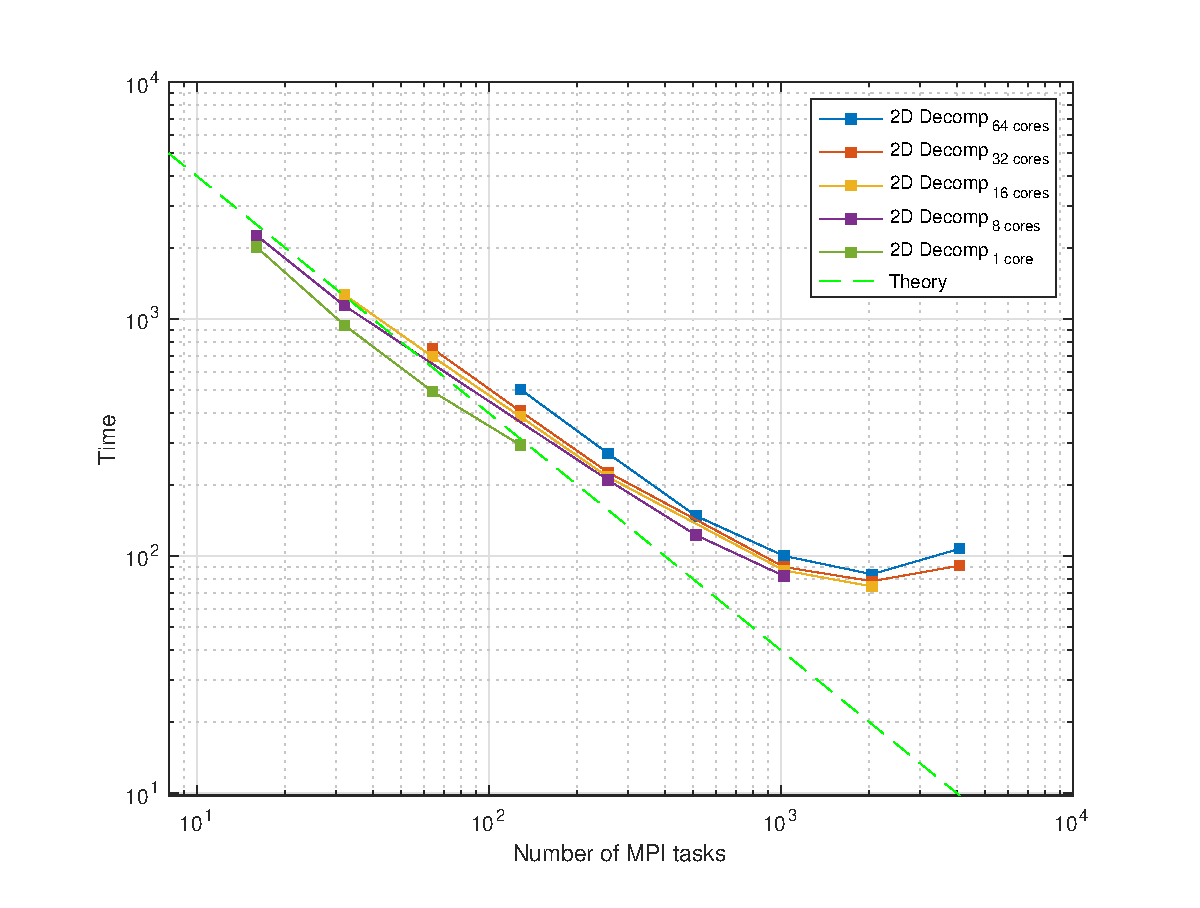
\includegraphics[scale=0.6]{grafici/5124}
\caption{Time scaling comparison for $512^3$ simulation}
\label{512:times}
\end{center}
\end{figure}

\begin{figure}
\begin{center}
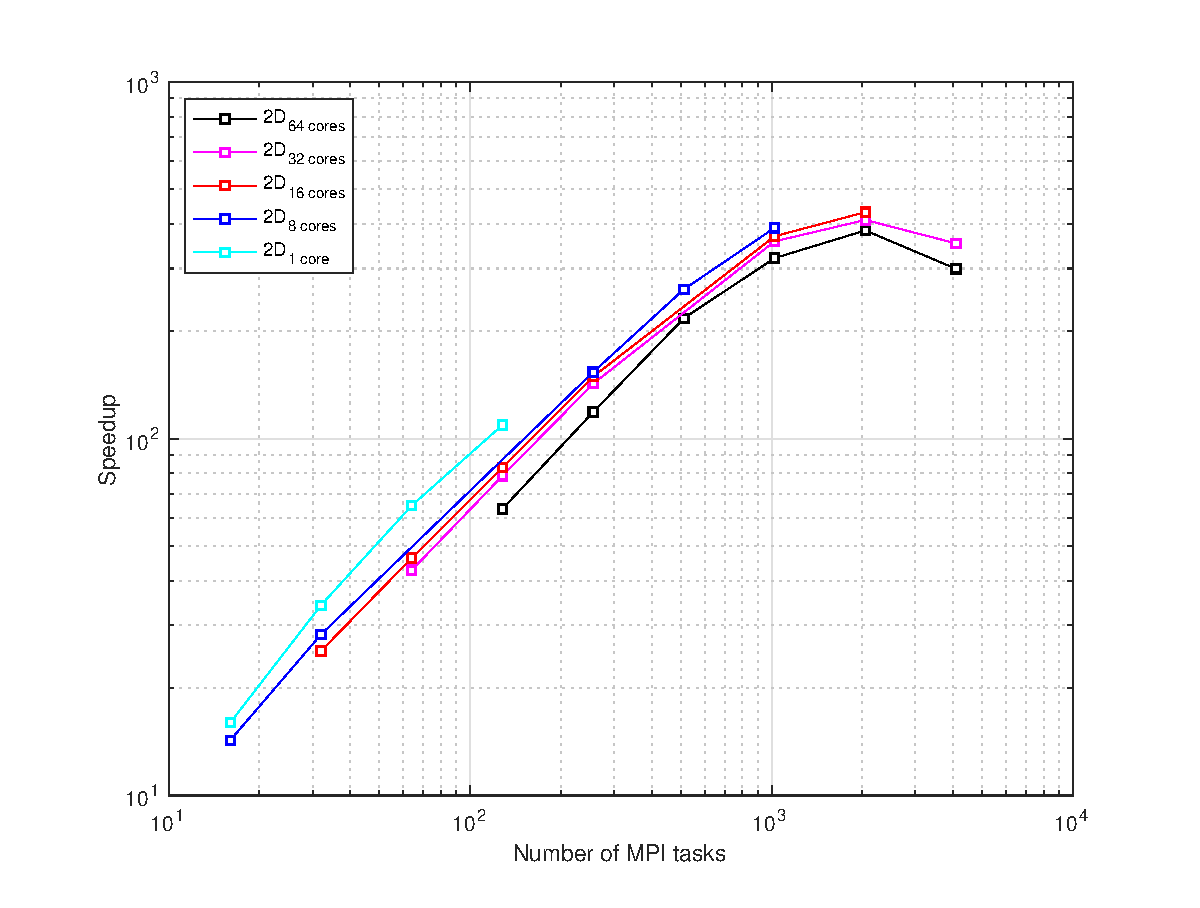
\includegraphics[scale=0.6]{grafici/5125}
\caption{Speedup factor comparison for $512^3$ simulation}
\label{512:perf}
\end{center}
\end{figure}

\begin{figure}
\begin{center}
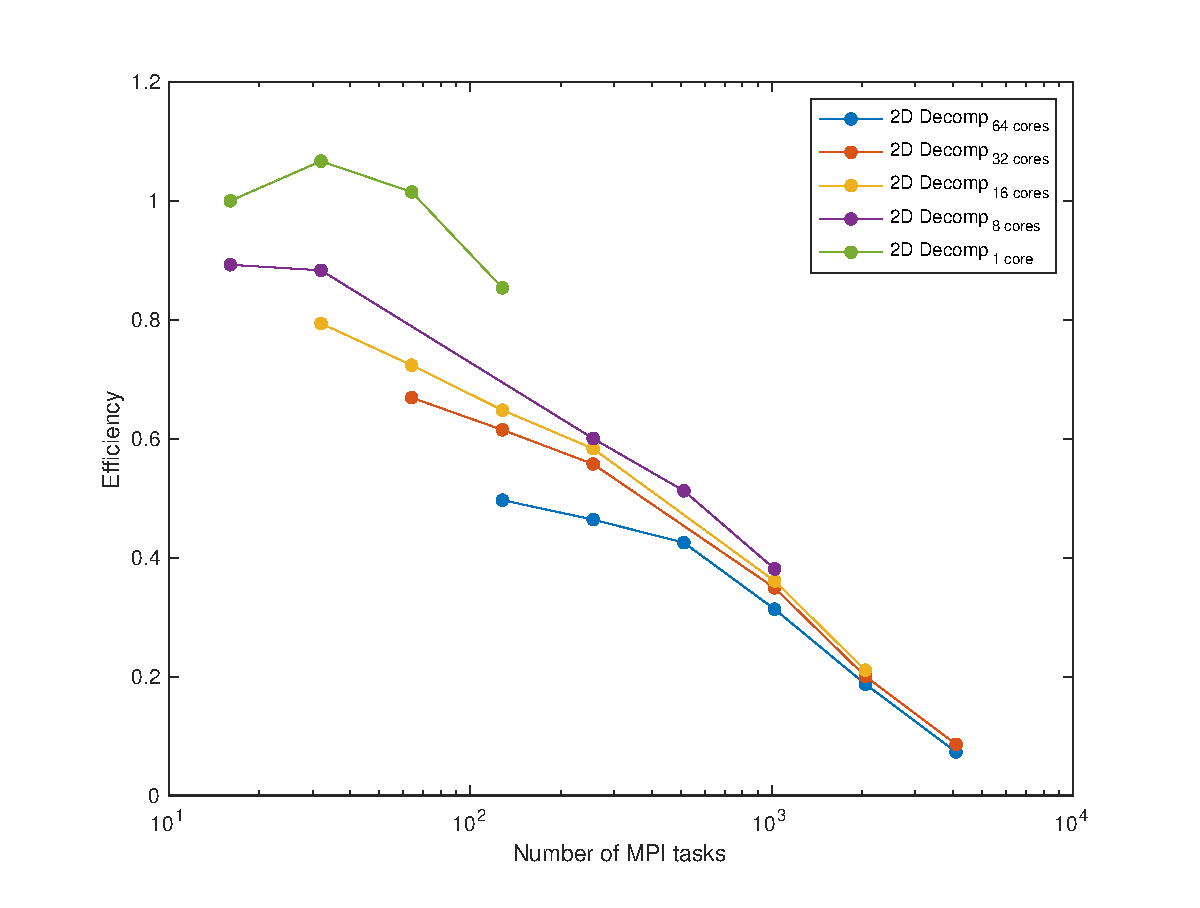
\includegraphics[scale=0.6]{grafici/5126}
\caption{Efficiency comparison for $512^3$ simulation}
\label{512:eff}
\end{center}
\end{figure}